\documentclass[11pt]{article}
\usepackage[utf8]{inputenc}
\usepackage{verbatim}
\usepackage{subfig}
\usepackage{makeidx}
\usepackage{listings}
\usepackage{color}
\usepackage{tikz}
\usetikzlibrary{arrows}
\usepackage{pgf}
\usepackage{fancybox}
\usepackage{verbatim}
\usepackage{wrapfig}
\usepackage{graphicx}
\usepackage{hyperref}

\newcommand{\bigstar}{\mathop{\Huge \mathlarger{\mathlarger{*}}}}


\definecolor{dkgreen}{rgb}{0,0.6,0}
\definecolor{gray}{rgb}{0.5,0.5,0.5}
\definecolor{mauve}{rgb}{0.58,0,0.82}

\lstset{ %
  language=Octave,                % the language of the code
  basicstyle=\footnotesize,           % the size of the fonts that are used for the code
  numbers=left,                   % where to put the line-numbers
  numberstyle=\tiny\color{gray},  % the style that is used for the line-numbers
  stepnumber=2,                   % the step between two line-numbers. If it's 1, each line
  % will be numbered
  numbersep=5pt,                  % how far the line-numbers are from the code
  backgroundcolor=\color{white},      % choose the background color. You must add \usepackage{color}
  showspaces=false,               % show spaces adding particular underscores
  showstringspaces=false,         % underline spaces within strings
  showtabs=false,                 % show tabs within strings adding particular underscores
  frame=single,                   % adds a frame around the code
  rulecolor=\color{black},        % if not set, the frame-color may be changed on line-breaks within not-black text (e.g. commens (green here))
  tabsize=2,                      % sets default tabsize to 2 spaces
  captionpos=b,                   % sets the caption-position to bottom
  breaklines=true,                % sets automatic line breaking
  breakatwhitespace=false,        % sets if automatic breaks should only happen at whitespace
  title=\lstname,                   % show the filename of files included with \lstinputlisting;
  % also try caption instead of title
  keywordstyle=\color{blue},          % keyword style
  commentstyle=\color{dkgreen},       % comment style
  stringstyle=\color{mauve},         % string literal style
  escapeinside={\%*}{*)},            % if you want to add LaTeX within your code
  morekeywords={*,...}               % if you want to add more keywords to the set
}

% If you add the above paragraph, the following can be used to alter the settings within the code:
% \lstset{language=C,caption={Descriptive Caption Text},label=DescriptiveLabel}


\title{Specialization Project \\ A closer look at deep artificial neural networks}
\author{Lars Andersen \\
Tormund S. Haus}
\date{\today}
\begin{document}
\maketitle
\newpage
\tableofcontents

\clearpage
\section{Introduction}

This report details the work done this semester in the specialization project.  The goal of the project was to investigate deep belief networks. Specifically, to implement a deep belief network (DBN), using restricted Boltzman machines (RBM) as building blocks.  Implementing these networks, based on scientific papers, proved to be a much larger challenge than expected.  Instead of writing about a failed implementation attempt, with entirely uninteresting results, this report will be a state of the art, where we take a look at some of the interesting technologies we've encountered throughout this semester.  At the beginning of the semester we had decided that these networks were interesting enough, in our eyes, that we wanted to work with them for a full year.  Thus, another goal of the project was to figure out what tasks these networks excel at, and where they come up short.  We then planned to use that knowledge to find a suitable project for the upcoming master thesis.

\section{Artificial Neural Networks}

An artificial neural network (ANN) is a computational abstraction based on how the brain works.  The human neurons, or those found in other animals, are incredibly complex in their own right.  The computational abstraction used makes no attempt at simulating the processes that affords neuronal activation and adaptation.  Instead, by less complex means, the functional workings of a neuron is simulated.  The standard abstraction used in ANNs is as follows:

\begin{enumerate}
 \item nodes.
 \item weighted connections between nodes.
 \item an integration function.  The most common integration function used sums the weighted output from all upstream neighbors.
 \item an activation function, which transforms the integrated input to an activation level for the neuron.  This activation level will be used as the output for the node, used by its downstream neighbors.
\end{enumerate}

\begin{figure}[htb]
  \centering
  \scalebox{0.6}
  {
    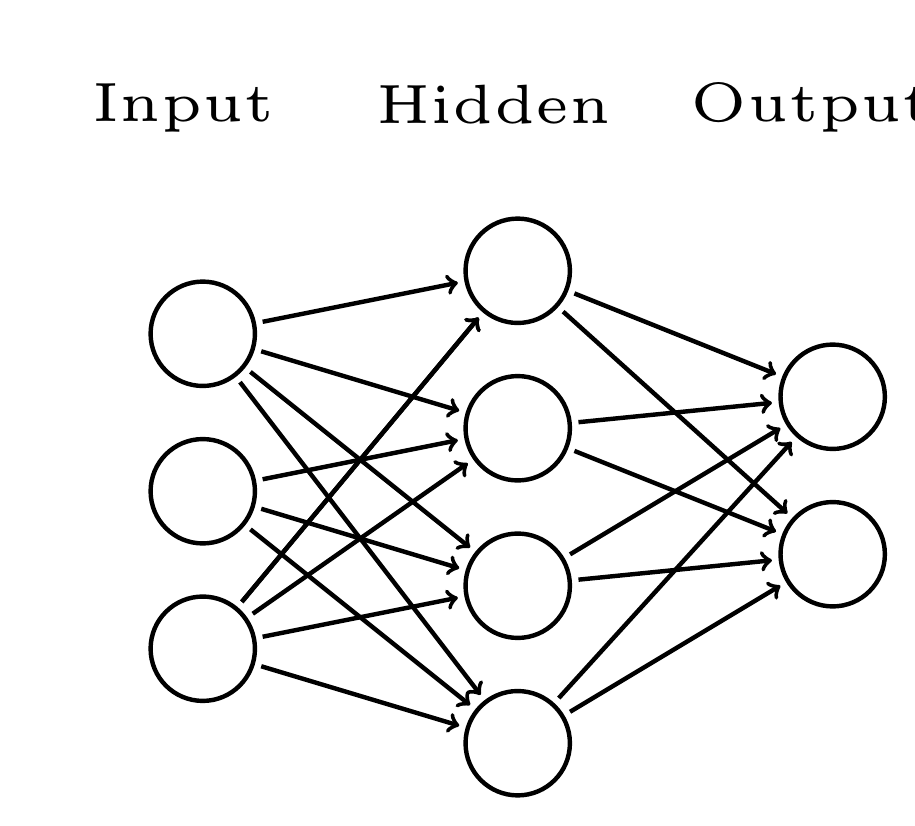
\begin{tikzpicture}[->,ultra thick,scale=4]
      \tikzstyle{every node}=[draw,shape=circle,scale=4]

      \node[draw=none,anchor=north,text width=0.1cm,font=\tiny] (input) at (-0.3,3.5) {Input};
      \node (v0) at (0,1.5) {};
      \node (v1) at (0,2) {};
      \node (v2) at (0,2.5) {};

      \node[draw=none,anchor=north,text width=0.1cm,font=\tiny] (input) at (0.6,3.5) {Hidden};
      \node (h0) at (1,1.2) {};
      \node (h1) at (1,1.7) {};
      \node (h2) at (1,2.2) {};
      \node (h3) at (1,2.7) {};

      \node[draw=none,anchor=north,text width=0.1cm,font=\tiny] (input) at (1.6,3.5) {Output};

      \node (o0) at (2,1.8) {};
      \node (o1) at (2,2.3) {};

      \draw (v0) -- (h0);
      \draw (v0) -- (h1);
      \draw (v0) -- (h2);
      \draw (v0) -- (h3);

      \draw (v1) -- (h0);
      \draw (v1) -- (h1);
      \draw (v1) -- (h2);
      \draw (v0) -- (h3);

      \draw (v2) -- (h0);
      \draw (v2) -- (h1);
      \draw (v2) -- (h2);
      \draw (v2) -- (h3);

      \draw (h0) -- (o0);
      \draw (h0) -- (o1);

      \draw (h1) -- (o0);
      \draw (h1) -- (o1);

      \draw (h2) -- (o0);
      \draw (h2) -- (o1);

      \draw (h3) -- (o0);
      \draw (h3) -- (o1);

    \end{tikzpicture}
  }
  \caption{A fully connected, feed-forward, artificial neural network with 3 input, 4 hidden and 2 output nodes.}
  \label{fig:ann}
\end{figure}

There are several ways to train an ANN, but the most common is to use an algorithm called \textit{backpropagation} to perform supervised learning.  The \textit{backpropagation} algorithm is so named because it propagates an error signal backward (from the output nodes toward the input nodes) through the network to assign blame and update connection weights.

Backpropagation can take a long time to converge to a solution, which may be a local optima and not a global one.  The computational complexity of backpropagation means that it can get prohibitively expensive to train large networks.  ANNs also typically grow in width rather than depth, when the model increases in complexity.  The reason for this is twofold:

\begin{enumerate}
\item Adding a new layer, of same size, adds a lot more connections.  In a fully connected, feed-forward, network adding another layer of N nodes will create an additional $N^2$ connections, whereas adding another node only adds $N$ new connections.
\item It is hard to meaningfully propagate an error signal through a very deep network.  If the weights are very small the gradient will be tiny at the start of the network.  If the weights are large, the gradients might be more reasonable, but we are likely to get stuck in a local minima of a highly multimodal landscape.
\end{enumerate}

In \cite{bengio09} Bengio makes a convincing case for why deep architectures are preferable to shallow ones.  The key point being that shallow networks are unable to efficiently encode certain functions.  These function are what the author calls \textit{highly varying functions}: functions where a piecewise-linear approximation of the function would require a large number of pieces.  In general this puts traditional ANNs at a disadvantage, and particularly so the ones being trained only with backpropagation.

\section{Restricted Boltzman Machines}

A Boltzman machine (BM) is a fully connected network of neuron-like units.  The connections are bidirectional and a stochastic process is used to determine whether a unit is on or not.  The number of connections in a BM makes them rather slow to train.  However, there exists an efficient learning algorithm\cite{hinton06} for a restricted BM (RBM): a BM where intra-layer connections are disallowed.

\begin{figure}[htb]
  \centering
  \scalebox{0.5}
  {
    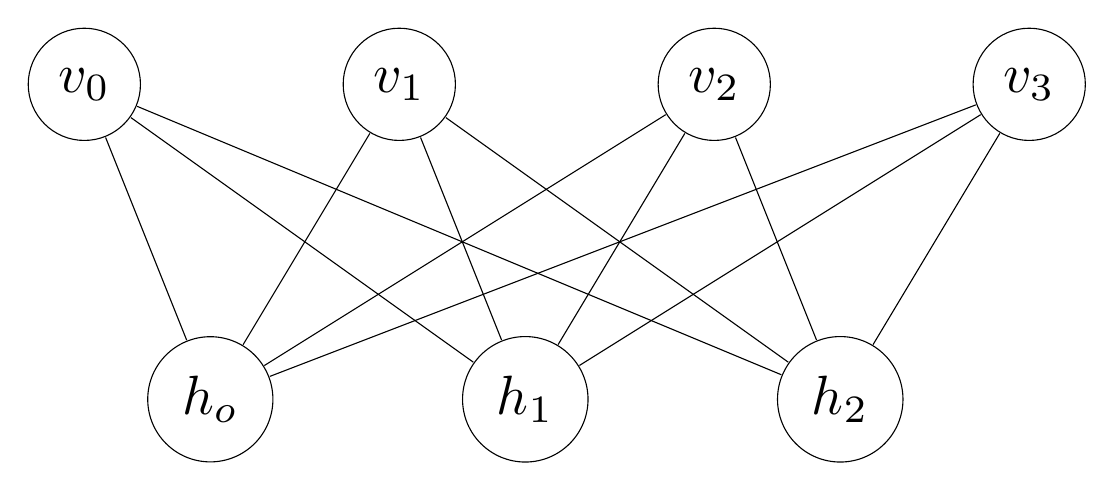
\begin{tikzpicture}[scale=4]
      \tikzstyle{every node}=[draw,shape=circle,scale=2]
      \node (h0) at (0.4,0) {$h_o$};
      \node (h1) at (1.4,0) {$h_1$};
      \node (h2) at (2.4,0) {$h_2$};

      \node (v0) at (0,1) {$v_0$};
      \node (v1) at (1,1) {$v_1$};
      \node (v2) at (2,1) {$v_2$};
      \node (v3) at (3,1) {$v_3$};

      \draw (v0) -- (h0);
      \draw (v0) -- (h1);
      \draw (v0) -- (h2);

      \draw (v1) -- (h0);
      \draw (v1) -- (h1);
      \draw (v1) -- (h2);

      \draw (v2) -- (h0);
      \draw (v2) -- (h1);
      \draw (v2) -- (h2);

      \draw (v3) -- (h0);
      \draw (v3) -- (h1);
      \draw (v3) -- (h2);
    \end{tikzpicture}
  }
  \label{fig:rbm}
  \caption{RBM with 4 visible and 3 hidden nodes.}
\end{figure}

Although RBMs might be unable to efficiently represent some distributions that can be compactly represented by a BM, it can be shown that an RBM, given enough hidden units, can represent any distribution\cite{le08}.  In addition, unless the RBM already perfectly models the training distribution, adding another hidden node (with correct weights and biases) always improves the model\cite{le08}.

The restricted Boltzman machine is so named because the energy metaphor is borrowed from physics.  In physics, the Boltzman distribution describes the fractional number of particles occupying a set of states with a given energy and temperature.  In our case, each input vector has a corresponding energy level.  During training this multi-dimensional energy landscape will be excavated to create ravines with clusters of training cases.  If the task is handwritten digit recognition then each digit class will map to a ravine in the energy landscape.  As in physics, the lower energy states are the most stable.

An RBM is not limited to doing discrimination, it is a generative model.  This means that the trained model can show its user what it believes in.  Sampling from the model is done using a process called Gibbs sampling.  To perform Gibbs sampling we clamp an input on the visible layer, which activates the hidden layer.  The hidden layer activation is in turn used to activate the visible layer.  If we repeat this process sufficiently many times it will converge.  We can start the process off by sending in an instance of training data, e.g an example of a handwritten 9, this will seed the model in a favorable way and the process of Gibbs sampling will converge quicker.  In practice this means starting the model off inside the energy ravine containing known examples of other 9s and then having the model wander around until it settles on a state.  If we start the sampling process off with a random input vector, the process will take longer to converge and we are unable to affect which area of the energy landscape is explored to find a stable energy state.

\section{Autoencoders}

An autoencoder takes an input $\mathbf{x} \in [0,1]^d$ and maps it--the encoding part--to a representation in the hidden units, $\mathbf{y} \in [0,1]^{d'}$, through a deterministic mapping:
 $\mathbf{y} = s(\mathbf{W}\mathbf{x} + \mathbf{b})$ where $s$ is a non-linear function, e.g. a function from the Sigmoid family.

The latent representation $\mathbf{y}$, or \textit{code}, is then mapped back--the decoding part--into a reconstruction $\mathbf{z} = s(\mathbf{W'}\mathbf{y} + \mathbf{b'})$.  The transformation is completely analogue with the encoding step and $\mathbf{z}$ has the same shape as $\mathbf{x}$.  Note that ' does not mean that the vectors or matrices are transposed in this context.

Optionally we can let $\mathbf{W'} = \mathbf{W}^T$.  Using this constraint we say that the weights are \textit{tied}.  This same terminology is used for RBMs as well and in that context it means that we are using the same weights for discrimination and generation.

The parameters of the autoencoder $W, b and b'$ are optimized such that the average reconstruction error is minimized.  One way to do this would be to use the \textit{squared error} to guide the weight changes.

\begin{figure}[htb]
  \centering
  \scalebox{0.6}
  {
    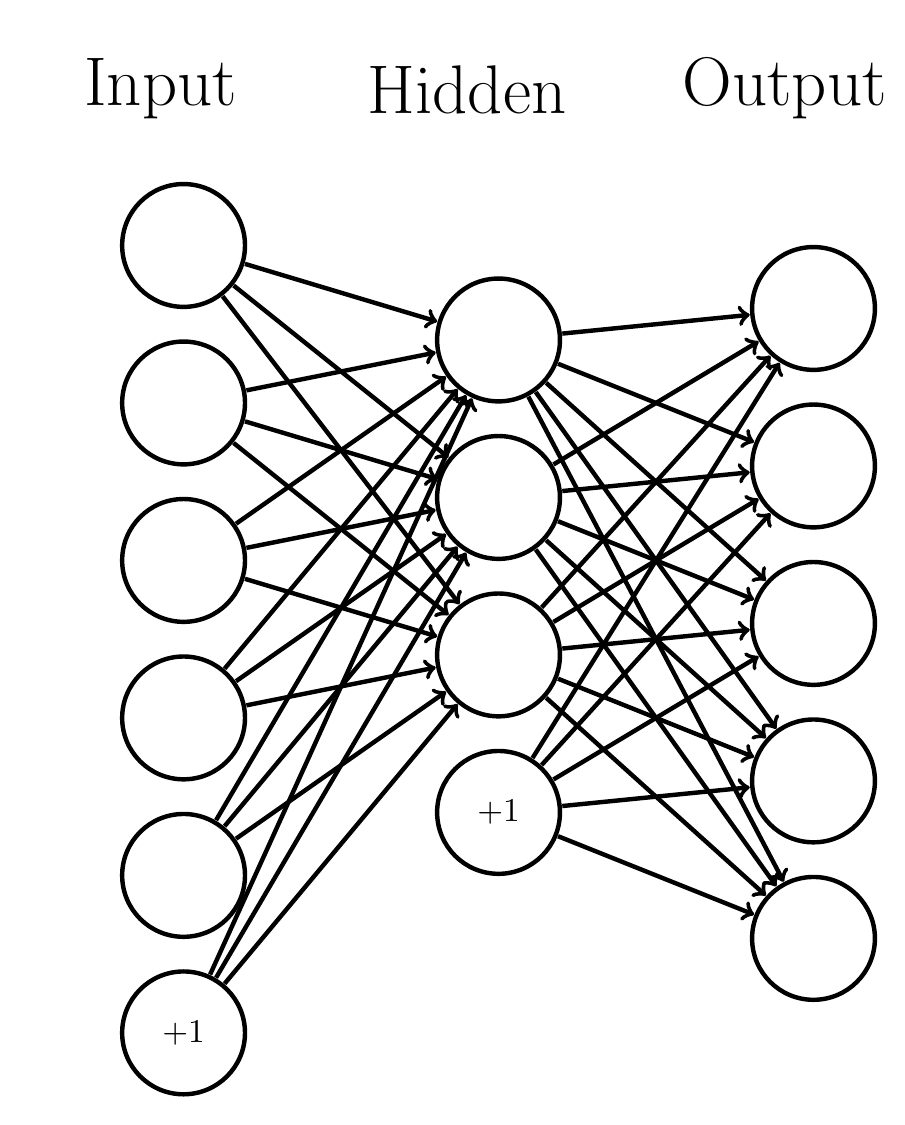
\begin{tikzpicture}[->,ultra thick,scale=4]
      \tikzstyle{every node}=[draw,shape=circle,minimum size=1.3cm,scale=4,text=,scale=0.3]

      \node[draw=none,anchor=north,text width=0.1cm,text=,scale=1,font=\huge] (input) at (-0.3,4.7) {Input};
      \node (v0) at (0,1.5) {+1};
      \node (v1) at (0,2) {};
      \node (v2) at (0,2.5) {};
      \node (v3) at (0,3) {};
      \node (v4) at (0,3.5) {};
      \node (v5) at (0,4) {};

      \node[draw=none,anchor=north,text width=0.1cm,text=,scale=1,font=\huge] (input) at (0.6,4.7) {Hidden};
      \node (h0) at (1,2.2) {+1};
      \node (h1) at (1,2.7) {};
      \node (h2) at (1,3.2) {};
      \node (h3) at (1,3.7) {};

      \node[draw=none,anchor=north,text width=0.1cm,text=,scale=1,font=\huge] (input) at (1.6,4.7) {Output};

      \node (o0) at (2,1.8) {};
      \node (o1) at (2,2.3) {};
      \node (o2) at (2,2.8) {};
      \node (o3) at (2,3.3) {};
      \node (o4) at (2,3.8) {};

      \draw (v0) -- (h1);
      \draw (v0) -- (h2);
      \draw (v0) -- (h3);

      \draw (v1) -- (h1);
      \draw (v1) -- (h2);
      \draw (v1) -- (h3);

      \draw (v2) -- (h1);
      \draw (v2) -- (h2);
      \draw (v2) -- (h3);

      \draw (v3) -- (h1);
      \draw (v3) -- (h2);
      \draw (v3) -- (h3);

      \draw (v4) -- (h1);
      \draw (v4) -- (h2);
      \draw (v4) -- (h3);

      \draw (v5) -- (h1);
      \draw (v5) -- (h2);
      \draw (v5) -- (h3);

      \draw (h0) -- (o0);
      \draw (h0) -- (o1);
      \draw (h0) -- (o2);
      \draw (h0) -- (o3);
      \draw (h0) -- (o4);

      \draw (h1) -- (o0);
      \draw (h1) -- (o1);
      \draw (h1) -- (o2);
      \draw (h1) -- (o3);
      \draw (h1) -- (o4);

      \draw (h2) -- (o0);
      \draw (h2) -- (o1);
      \draw (h2) -- (o2);
      \draw (h2) -- (o3);
      \draw (h2) -- (o4);

      \draw (h3) -- (o0);
      \draw (h3) -- (o1);
      \draw (h3) -- (o2);
      \draw (h3) -- (o3);
      \draw (h3) -- (o4);

    \end{tikzpicture}
  }
  \caption{An autoencoder with 5 input, 3 hidden, and 5 output nodes.  Bias nodes are included in the input and hidden layer.}
  \label{fig:ae}
\end{figure}

The gist of it all is that the autoencoder does its best to replicate the input.  The autoencoder drawn in \ref{fig:ae} is perhaps the most common type, where the layer(s) between the input and output layer has a lower dimension.  This will force the autoencoder to learn a compressed representation of the input vector, which it then uses to create the output.  Intuitively, one would think that if the intermediary representation was of the same, or higher dimension, the autoencoder would simply learn the identity function.  Bengio et al. tackled this question in \cite{bengio07} and found that autoencoders with non-decreasing layer sizes also generalize well.  They do, however, speculate that this might be explained by their use of stochastic gradient decent and weight decay.  In other words in the general case, we might risk learning the identity function.

A final point about autoencoders is worth mentioning: if the autoencoder is built using only linear hidden units, i.e $\mathbf{s}$ is picked from the family of linear functions, then training the autoencoder is equivalent to performing principal component analysis (PCA).

\subsection{Denoising Autoencoders}

The denoising autoencoder is a stochastic version of the autoencoder.  Stochastic because the input is corrupted through some stochastic process.  The non-corrupted input is however used as a target for reconstruction.  The corruption process is performed by setting some, but not more than half, of the inputs to zero.  The denoising autoencoder is thus trying to perform two tasks:
\begin{enumerate}
\item Encode the input
\item Undo the effect of corruption
\end{enumerate}

The motivation behind the denoising autoencoder is to attempt to answer the question ``what properties should we demand of a good representation?''  Many come to mind, but the one investigated in \cite{bengio07} is ``robustness to partial destruction of the input''.  For high dimensional inputs, with redundant information (like in images), the representation is likely to depend on many factors along many dimensions and therefore likely be recoverable from partial observations.  The obvious example, mentioned in the paper, is our human ability to recognize objects which are partially covered up or corrupted in images.

\section{Deep Belief Networks}

\subsection{Using RBMs}

A deep belief network (DBN) can be created by stacking multiple RBMs.  When the input vector is processed by the first RBM its output is a new representation of the data.  This new representation can then be used as input to the RBM in the layer above.  The hope is that each RBM is better able to represent the data, by creating useful abstractions or simply removing noise.  In \cite{hinton06} Hinton shows that adding more layers in a DBN will always improve the model.  The use of the \textit{contrastive divergence} learning algorithm voids this guarantee, but it increases our confidence in the method to know that we can always improve the model by being patient enough in training each layer.

The way to train a DBN is to use a greedy layer-wise training algorithm.  Each layer, consisting of one RBM, is trained before we move on to train the next one.  By freezing the weights after we're done training each RBM we miss out on any positive effect that might be had by the coordinated tuning of weights in two, or more, adjacent layers.  One way to overcome this inefficiency of the greedy training approach is to fine-tune the network after the greedy training phase is done.  Fine-tuning can be done using the well-known backpropagation algorithm, or some other algorithm for gradient decent.  By seeding the backpropagation algorithm with a promising state the following problems encountered using backpropagation in deep networks are solved\cite{hinton06reducing}:
\begin{enumerate}
\item If the initial weights are small the gradients in the earlier layers will be tiny and weight changes ineffectual.
\item If the initial weights are large the network typically gets stuck in poor local minima.
\end{enumerate}

When the initial weights are just right, gradient decent works quite well.

\subsection{Using autoencoders}

A deep belief network can also be created by stacking multiple (denoising) autoencoders.  The process is entirely analogous to the situation with RBMs.  First the network is trained unsupervised pre-training and then fine-tuned using an algorithm like backpropagation.  In \cite{bengio07} DBNs using stacked denoising autoencoders were found to perform as good, or better, than DBN networks of stacked RBMs, on the MNIST dataset.

Another related type of network can be found in \cite{hinton06reducing}.  In this paper, which is about dimensionality reduction of data using ANNs, a three RBMs of dimensions 2000-1000, 1000-500 and 500-30 are trained using a greedy unsupervised approach, as discussed earlier.  The weights are then \textit{unrolled} to create a new network of structure 2000-1000-500-30-500-1000-2000, which is then fine-tuned using backpropagation.  This network is itself an autoencoder and is referred to as a \textit{deep autoencoder}.

\section{Convolutional Neural Networks}

The first convolutional neural network (CNN) was described in Fukushima's seminal paper on the Neocognitron\cite{fukushima}.  The modern terminology was not used in this paper, but the key principles are the same.  Inspired by the work done by Hubel and Wiesel, on the cat's visual cortex\cite{hubel}, the goal was to create a biologically plausible ANN to explore image recognition (specifically, images of digits).  One of the key insight in Fukushima's paper is that feature detection should be modular and location invariant: we should re-use the same structure in order to detect one feature in the image, regardless of the coordinates of the feature within the image.  In implementational terms, in regard to an ANN, this means we should re-use weights to detect features.

\subsection{What is convolution}

The term convolution is taken from the field of image processing.  In image processing, to convolve an image, with a filter (also called kernel), means to apply the filter to each pixel in the image.  A filter is created by defining weights of neighbor pixels to a center pixel.  The product of weights and pixel values are then summed to find the new value of the center pixel.  So, if our filter is a 3x3 identity matrix, the new value of the center pixel will be the sum of the pixel values of its south-east and north-west neighbor.  A typical use-case for convolution in image processing is edge detection.

The use of convolution in ANNs is quite analogous: the filter is a feature detector. The sum, of products of pixel values and weights, is not used to create a new center pixel, but instead expresses the probability that the feature being detected is present at the given location in the picture.  Thus, the result of convolving an image with a filter is a matrix of probabilities, a feature map if you will.  By convolving the image with many filters we can create several feature maps.  If we denote the k-th feature map at a given layer as $h^k$, which is determined by the weights $W^k$ and bias $b_k$ then the feature map $h^k$ is:

\begin{displaymath}
  h^{k}_{ij} = \sigma((W^k * x))_{ij} + b_k
\end{displaymath}

Where * means matrix convolution, and not multiplication, and $\sigma$ is some non-linear function, typically selected from the sigmoid family.

\subsection{Pooling}

Pooling is another important key component of CNNs.  There are various types of pooling, but the most common ones are max and mean-pooling.  To perform max pooling the feature maps are partitioned into non-overlapping rectangles, and for each sub-region, the output is the maximum value.  In other words, how likely the feature is to be present in the sub-region.

Max pooling serves two purposes:

\begin{enumerate}
\item Reduction of computational complexity, for upper layers of the network.
\item Provide translational and deformational invariance.
\end{enumerate}

Since max pooling provides increased robustness, in terms of the position of features within an image, it has proven to be a good way of reducing the dimensionality of the intermediary representations.

If we refer back to the work done by Hubel and Wiesel the convolution step used for feature extraction corresponds to the work done by the \textit{simple cells} and the pooling operation to the work done by the \textit{complex cells} found in the visual area V1.

\begin{figure}[htb]
  \centering
  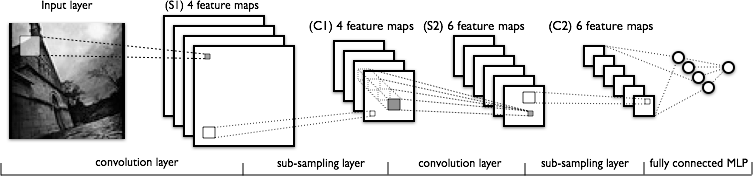
\includegraphics[width=\textwidth]{mylenet.png}
  \caption{Model of LeCun's convolutional network LeNet}
  \label{fig:mylenet}
\end{figure}

In figure \ref{fig:mylenet} we get a descriptive view of how a CNN works.  In layer $\mathbf{S1}$ we can see 4 feature maps, describing the probabilities that 4 different features are present at various locations of the image.  $C1$ is a sub-sampling layer, where the sub-sampling operator is max pooling.  $\mathbf{C1}$ then feeds into $\mathbf{S2}$ which creates new feature maps based on more abstract features.  At the very top of the network, in LeNet, we find a fully connected multi-layer perceptron (MLP) with logistic regression.

In figure \ref{fig:mylenet} we can also see how the receptive field of each detector increases in size as we move toward the to of the network.  The first convolutional layer uses filters with receptive fields which are say 4x4 in size, the receptive field of \textit{simple cells}.  The max pooling layer then looks at say a 3x3 region of the feature map and in terms of the original image each \textit{complex cell} has a receptive field of $(4 + 3 - 1)^2$ pixels of the input image, or $(rank(\mathbf{S1}) + rank(\mathbf{C1}) - 1)^2$.  Where $rank(A) = n\ \Leftrightarrow$ A is an $N\times N$ matrix.

\subsection{Use of convolutional neural networks}

For a long time, the only viable option for creating deep artificial neural networks was to build a convolutional network.  Deep fully connected networks trained using backpropagation were computationally intractable, but the CNNs were not.  There are several reasons for this:

\begin{enumerate}
\item The filters are small.  It is therefore not very computationally intensive to find the correct weights used to detect a feature.
\item The complexity of the network can be controlled by choosing how many features to use at each level.
\item The sub-sampling layers do not need training at all.
\item The sub-sampling layers provide a reduction in dimensionality, decreasing the computational load.
\item Shared weights, in the filters, provide a lot of bang for the buck.
\end{enumerate}

The ideas used in convolutional networks are sound, so they have not fallen out of favor.  On the contrary, they are very scalable and produce state-of-the-art results.  There are several ways to put any additional computational power to good use:
\begin{itemize}
\item Detect more features.
\item Adjust the size of the filters.  Smaller filters are more computationally intensive, but afford a higher level of detail.
\item Add more layers.
\end{itemize}

CNNs are primarily used in machine vision, because the statistics of the image is the same everywhere (a given feature is equally likely to appear anywhere in the input image) making translational invariance very important.

\subsection{Multi-scale Convolutional Network}

In \cite{farabet} a CNN is created which is scale invariant, for the purpose of scene parsing.  The scene parsing task consist of identifying and labeling the objects making up an image.  In practice means assigning an object class to each pixel e.g. sky, road or person.

The importance of scale invariance, in regards to this task, is obvious: it is desirable for a ``small person'', i.e. a person in the background of the image, to be identified as a person even if the training set only contains images where the persons appear in the foreground.

The problem of scale invariance can be solved by extending the concept of weight sharing over locations, to sharing weights over scales.  The weights are shared among different CNNs.  During classification the image is scaled--3 different sizes are used in the paper--and each version is sent to one CNN.  The final feature vector represents the concatenation of the feature vectors from the 3 CNNs.

\subsection{Multi-column deep neural network}
In \cite{ciresan} and \cite{ciresan2} a multi-column deep convolutional network (MCDNN) is used to improve the state-of-the-art on several classification tasks using e.g. the MNIST and NORB dataset.  Traditional CNNs, with randomly initialized weights, are initialized and all of them trained either one the same training sets or distorted variants.  The final classification is done with a democratic vote between the columns.

Max pooling is used to create a winner-takes-all effect where only the winner neurons receive training.  The authors argue that this represents a biologically plausible mechanism where the ever decreasing number of changes per time interval lead to reduced energy consumption. TODO insert image.

In order to speed up training the entire system is optimized to run on GPUs. The authors estimate that using GPUs leads to an increase in computational power of around 50-100x.  Furthermore, this additional processing power removes the need for pre-training completely.  The network is trained through no other means than an online version of backpropagation (weight updates after each training case).

This system is the first one able to achieve human-competitive results on the MNIST dataset.  Humans typically reach error levels of 0.2\%, not much better than the 0.23\% achieved by MCDNN.

\subsection{Convolutional Deep Belief Network}

In \cite{lee} a convolutional deep belief network is created.  Recall that what separates a deep belief network from other kinds of deep networks is that it is a generative model, able to generate observable data.  There are several reasons that make the combination of convolutional and deep belief networks desirable:
\begin{itemize}
 \item The effect of training on unlabeled data is greater in belief networks.
 \item The lack of mechanisms like weight-sharing and pooling for RBM based deep belief networks makes training on large input images computationally intractable in practice.
 \item Deep belief networks are able to do inference both top down and bottom up, i.e. they are able to infer missing data.
\end{itemize}

The building blocks in the deep convolutional belief network is the convolutional RBM (CRBM).  A CRBM is similar to a regular RBM, but with a few key differences:

\begin{itemize}
 \item The hidden layer of the RBM is really two layers:
   \item \begin{itemize}[(a)]
           \item A \textit{detection layer} which performs convolution.
            \item A \textit{a pooling layer} which performs pooling.
          \end{itemize}
 \item The detection layer has $\mathbf{K}$ groups, made up of $\mathbf{N_H \times N_H}$ hidden units.  If we are detecting $\mathbf{K}$ features consisting of $\mathbf{N_W \times N_W}$ ``pixels''.
 \item To sample from the visible units we use convolution instead of propagating the activation of the input layer.
\end{itemize}

Max-pooling was only intended for feed-forward architectures so a new variant called probabilistic max-pooling is used.  A regularization step is also used in order to force sparsity, because the model in the paper is overcomplete.

\section{Conclusion}

Various types of deep neural networks are at the bleeding edge of many classification tasks.  There are many factors which make them attractive classifiers, but chief among them are perhaps:
\begin{enumerate}
\item The ability to train on raw data, avoiding the need for complex feature engineering.
\item Scalability, combined with the ever-increasing availability of computational resources.
\item The ability to tackle a diverse range of tasks without use of explicit domain knowledge.
\item Performance can be improved, greatly, by doing unsupervised training on readily available unlabeled data.
\end{enumerate}

We have focused on image processing, partly because we find this application most interesting, but also because the literature itself favors this task.  The reason for this favoritism is not only due to flights of fancy, but because certain mechanisms, like weight-sharing and max-pooling work very well when the input data is contiguous (e.g. as image data is, or a contiguous sound wave).  Another reason is that the imaging tasks represent real challenges due to both the size and high dimensionality of the input data, making the task a worthy research subject.

The obvious value of any improvements to tasks like machine vision has lead to a situation where there is a lot more back and forth between academia and industry than was is usual for AI research.  Google is currently using deep belief networks to power their voice-to-text engine found in the Android operating system.  In \cite{ng} Andrew Ng teamed up with Google to run deep learning, on an object recognition task, using a cluster of 1000 machines for a total for 16000 cores.  The model has one billion connections.  Deep networks also powered Microsoft's recent demonstration of real-time translation of speech, where the speech was synthesized using a model of the speaker's own voice.  The net result was a presentation where the speaker spoke English and the audience hear the speaker speak Chinese, in his own voice.  The demonstration of this technology is well worth a \href{http://www.youtube.com/watch?v=Nu-nlQqFCKg}{look}.

The short distance between theory and practice for this kind of technology, makes it especially interesting to work with.

\bibliographystyle{plain}
\bibliography{references}

\end{document}
